\section{Błyskawiczny makaron w sosie orzechowym}
\bigskip
\small
\begin{minipage}{0.45\textwidth}
    \noindent \textbf{Czas:} 10 minut \\
    \textbf{Poziom trudności:} łatwy
\end{minipage}
\begin{minipage}{0.45\textwidth}
    \noindent \textbf{Ilość sprzątania:} minimalna\\
    \textbf{Wymagany mysi sprzęt:} blender (opcjonalnie)
\end{minipage}
\normalsize
\vspace{0.5cm}

\begin{multicols}{2}

\subsection*{Składniki}
\begin{itemize}
    \item porcja makaronu ryżowego (można też użyć pszennego)
    \item 2 łyżki masła orzechowego
    \item 1 duży lub 2 małe ząbki czosnku, przeciśnięte przez praskę
    \item 1 łyżka sosu sojowego
    \item 1/2 - 1 łyżka ostrego sosu typu sriracha
    \item odrobina wyciśniętego soku z cytryny
    \item 1 łyżka miodu lub cukru
    \item 5 łyżek wrzątku lub wody spod makaronu
    \item 1 łyżeczka oleju sezamowego
\end{itemize}

\columnbreak

\begin{figure}[H] \centering
 \fbox{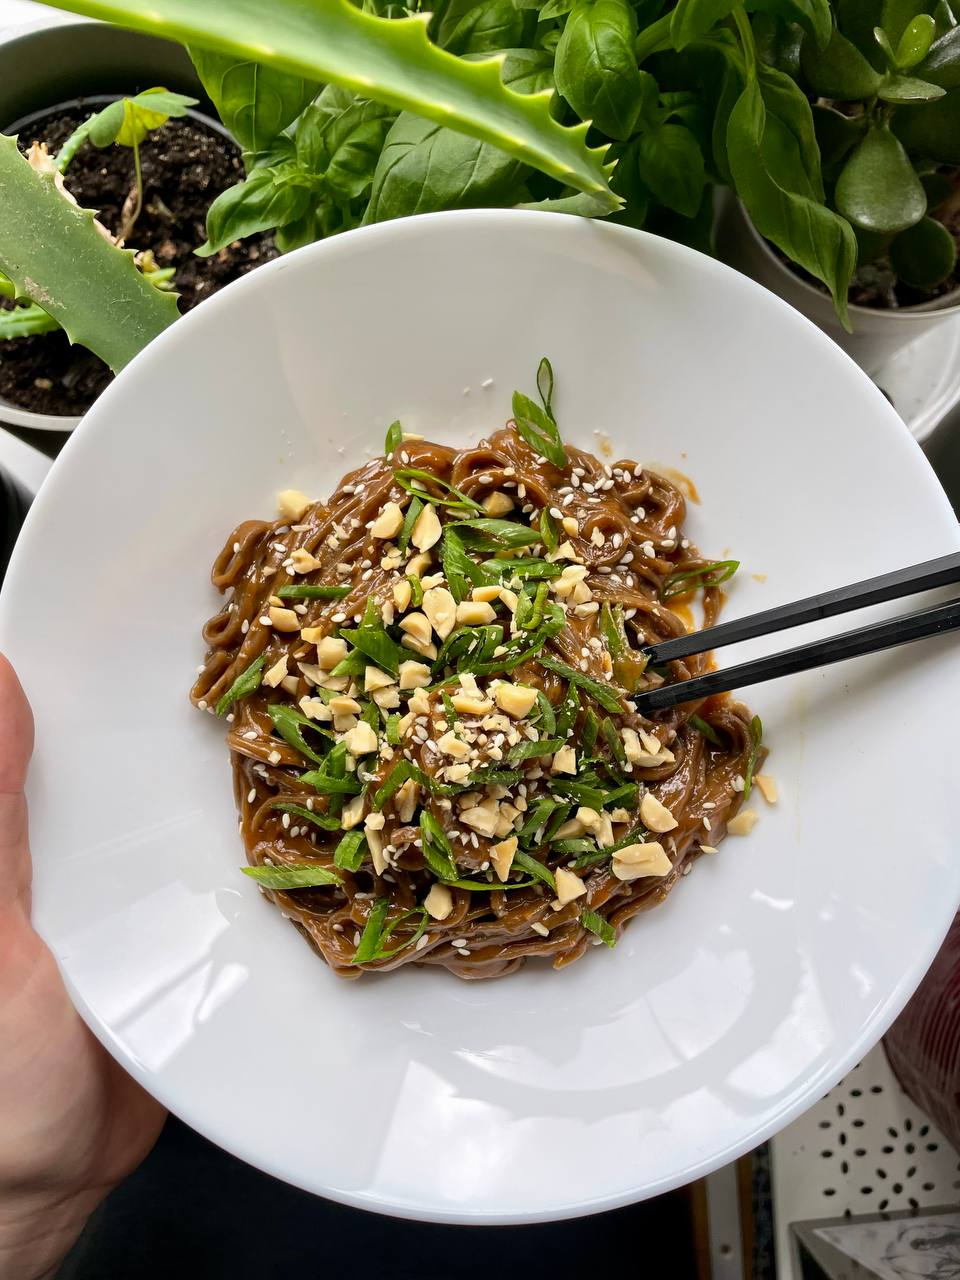
\includegraphics[width=0.35\textwidth]{images/makaron-orzechowy.jpg}}
\end{figure}

\end{multicols}

\vspace{0.5cm}

\subsection*{Instruktaż}
\begin{enumerate}
    \item Zagotować osoloną wodę na makaron i gotować według instrukcji na opakowaniu.
    \item W międzyczasie połączyć resztę składników w niewielkiej miseczce i dokładnie wymieszać lub zblendować na gładki sos.
    \item Makaron odcedzić i przełożyć z powrotem do garnka. Wymieszać z sosem i ewentualnie podgrzać.
\end{enumerate}

\vspace{0.5cm}

\small \subsection*{Propozycja podania} Z orzeszkami ziemnymi, z posiekaną zieloną cebulką, z nasionkami sezamu.

\vspace{0.3cm}

\subsection*{Dodatkowe uwagi} W celu zwiększenia ilości białka w daniu do makaronu można dodać usmażone na chrupko tofu bądź kawałki kurczaka.

\newpage
